\section{Введение}

\subsection{Требования к ядру}
Рекомендуется использовать ядро Linux 4.9 (релиз в декабре 2016 года) или более
новое. Некоторые параметры конфигурации ядра должны быть включены.
Вот эти параметры: \\
\ci{CONFIG\_BPF=y}
\ci{CONFIG\_BPF\_SYSCALL=y}
\ci{CONFIG\_BPF\_JIT=y}
\ci{CONFIG\_HAVE\_EBPF\_JIT=y}
\ci{CONFIG\_BPF\_EVENTS=y}

\subsection{Установка в Ubuntu}
\cn{sudo apt-get update}

\noindent bpftace: \\
\cn{sudo apt-get install bpftrace}

\noindent bcc: \\
\cn{sudo apt-get install bpfcc-tools linux-headers-\$(uname -r) }

\cn{\# ls /sbin/*-bpfcc}

\subsection{Схема BCC}
\url{https://github.com/iovisor/bcc}

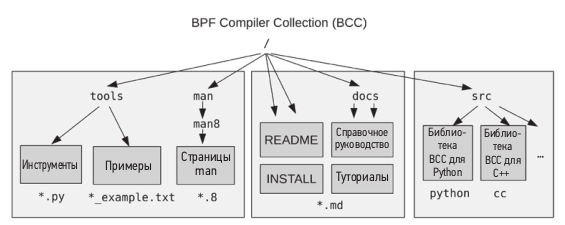
\includegraphics[width=0.8\linewidth]{structure_bcc.png}

\subsection{Схема bpftrace}
\url{https://github.com/bpftrace/bpftrace}

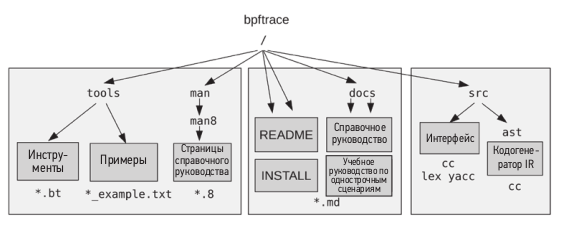
\includegraphics[width=1.0\linewidth]{structure_bpftrace.png}

\subsection{Полезные ссылки}

\noindent BPF Performance Tools - Материалы из книги Brendan Gregg: \\
\indent \url{https://github.com/brendangregg/bpf-perf-tools-book/tree/master} \\

\noindent Docs от разработчиков Bpftrace: \\
\indent \url{https://github.com/bpftrace/bpftrace/tree/master/docs} \\

\noindent BPF на сайте Brendan Gregg: \\
\indent \url{https://brendangregg.com/ebpf.html} \\

\noindent Статья на хабре: \\
\indent \url{https://habr.com/ru/articles/542560/}
